%% The following is a directive for TeXShop to indicate the main file
%%!TEX root = ../diss.tex

\chapter{Oxygen enhanced MRI - Applications 3}
\label{ch:oemri3}

% ======================================================================
\section{Introduction}
% ======================================================================

Dynamic oxygen enhanced MRI (dOE-MRI) has recently been proposed by our group to assess tumour oxygenation in vivo using MRI~\cite{Moosvi:2018ca}. 
This technique measures T1-weighted changes in tissues in response to a cycling oxygen challenge, with the responsive signals detected using independent component analysis (ICA). 
Briefly, oxygenation can be assessed \emph{in vivo} by administering a simple gas challenge (switching between two-minute periods of medical air and 100\% O$_2$) during the dOE-MRI scan and then using ICA to extract the tissue response.
ICA is a blind-source separation algorithm that separates multiple signal sources by maximizing statistical independence of individual components~\cite{Hyvarinen:2000vk}.
Various flavours of oxygen-enhanced MRI (OE-MRI) have been proposed but all essentially leverage the paramagnetic properties of inhaled oxygen.
White et al. has shown that OE-MRI may be very relevant in developing prognostic factors to predict tumor response to hypofractionation by stratifying tumors that may benefit from oxygen breathing during irradiation~\cite{White:2016fz}.
In this study, we apply dOE-MRI to mice bearing tumour xenografts to assess the effect of a common antiangiogenic agent.

Aberrant angiogenesis, poor blood perfusion, a chaotic vascular network all limit oxygen delivery to cells and contribute to formation of hypoxic regions in tumours.
The binding of vascular endothelial growth factors (VEGF) to the VEGF receptor is a key driver of angiogenesis.
Bevacizumab (Avastin) is a monoclonal antibody that binds VEGF extracellularly, preventing the interaction of of VEGF to its receptors and inhibits angiogenesis. 
Avastin has been used clinically to treat breast, colon, colorectal, lung, brain, ovarian, cervical, and other cancers~\cite{AvastinIndications}\todo{cite Genentech}%https://www.gene.com/download/pdf/avastin_prescribing.pdf]. 
VEGF ablation has been shown to at least temporarily reduce vascular permeability and increase tumour oxygenation in some models~\cite{OConnor:2012iea}\todo{this review has lots of relevant refs, better to cite directly than a review}. 
We hypothesized that dOE-MRI with groupICA can detect VEGF ablation-induced changes to oxygenation of SCCVII tumours 48 hours following treatment.

% ======================================================================
\section{Methods}
% ======================================================================
\subsection{Animals}
Female NRG (NOD rag gamma) mice were implanted with murine squamous cell carcinoma (SCCVII; 5x10$^5$ cells in 50$\mu$l serum-free media; cells provided by Dr. J. Evans) in the dorsal subcutaneous region.
Approximately X \todo{how many days?} days later, tumours were imaged when their largest diameters reached approximately 8-10 mm.
All mice were injected with 60 mg/kg pimonidazole hydrochloride (HypoxyProbe) 30 min prior to imaging to label hypoxic cells and were euthanized within 15 min of imaging completion.
Mice were anesthetized with isoflurane using 1.5-2.0\% isoflurane for the duration of MR imaging sessions until euthanasia, and were positioned supine on the custom surface coil apparatus.
Throughout the imaging session, a small animal monitoring system (SAII Instruments, Stony Brook, NY, USA) was used to monitor respiration rate, varying between 80-100 breaths per minute, and body temperature, maintained at 36.8 $\pm$ 0.5$^\circ$C using a continuous airflow heater. 
Tumors were embedded and frozen in optimum cutting temperature medium (OCT; Tissue-TEK).
All animal experimental procedures were carried out in compliance with the guidelines of the Canadian Council for Animal Care and were approved by the institutional Animal Care Committee.

\subsection{Immunohistochemistry}
Co-planar MRI slices and histological sections were obtained by imaging perpendicular to the longest tumour axis in MRI and serial-step 10 $\mu m$ cryosections were cut at 0.5-mm intervals in the same plane.
Slides were then fixed in acetone-methanol for 10 min and whole sections were immunohistochemically stained~\cite{Kalra:2017is} for CD31 (PECAM; visualized using secondaries labeled with Alexa 647nm) to label blood vessels, and for pimonidazole (HypoxyProbe-1; visualized using secondary labeled with Alexa 546nm) to label hypoxic cells. Sections were then stained using Hoechst 33342 (bisbenzimide) to label all cell nuclei.
Whole-tumor sections were imaged using a robotic fluorescence microscope (Zeiss Axioimager Z1), a cooled, monochrome CCD camera (Retiga 4000R; QImaging), a motorized slide loader and x-y stage (Ludl Electronic Products) and customized ImageJ software~\cite{Collins:2007jr}. 
Adjacent microscope fields of view were tiled such that images of entire tumour cryosections were captured at a resolution of 1.5 $\mu m$/pixel. 
Using anatomical landmarks and accumulated thicknesses of serial-step sections as estimates of distances from the edges of whole tumours, sections were chosen to match the MR slices. 
ImageJ and user-supplied algorithms were used to super impose digital images which were then manually cropped to tumour tissue boundaries with staining artifacts removed. 
A threshold was applied to images to identify positive pimonidazole staining, and the number of positive pixels was determined as a percentage of the total number of pixels in the tumour image. 
Overlaid greyscale images were converted to false colour for visualization with pimonidazole as green and CD31 as magenta~\todo[backgroundcolor=green]{need to make sure final colours are consistent}.

\subsection{MR Imaging}
Imaging was performed using a 7T scanner (Bruker Biospec) with a transmit quadrature volume coil and a custom built surface receive coil. 
An axial RARE image was acquired to localize the tumour (TE/TR=10.7/4250ms, RARE factor 8) and a T$_1$ map was acquired using the Look-Locker method.
Dynamic oxygen enhanced MRI (dOE-MRI) scans were acquired with a 2D multi-slice FLASH-based sequence for a total scan time of about 14 minutes.
During the dOE-MRI scan, breathing gas was alternated between medical air and 100\% oxygen every 2 minutes using a 3-channel gas mixer (CWE, Philadelphia, USA) for a total of 3 air-oxygen-air cycles.
All scans were acquired with the same spatial resolution and geometry and an experienced operator outlined the tumour on each slice of the RARE image to construct the region of interest (ROI) for each animal and then transferred to all other scans.

\subsection{dOE-MRI Analysis}
A suite of in-house software was developed using the python machine learning library scikit-learn~\cite{Pedregosa:2011tv}, specifically \texttt{sklearn.decomposition.FastICA} based on the technique described by Hyvarinen~\cite{Hyvarinen:2000vk}.
The FastICA algorithm is applied to serially acquired T$_1$W images and the output is a paired set of components and weighting factors for each voxel in the dataset.
The deflation-based FastICA (python package scikit.sklearn v0.17.1) was used to analyze the data. 
Extracted independent components are not ordered and while the component selection can be automated, in this study an observer was assigned to select the appropriate component.
The number of independent components for each imaging session was chosen by the operator and ranged from 4-9 to ensure the cyclic behaviour of the T$_1$W signal intensity corresponding to the gas challenge appeared in only one component. 
The dOE-MRI maps were obtained by dividing the ICA weighting-factor maps by the mean signal-intensity maps to obtain a spatial map for the strength of a particular voxel's contribution to the component of interest.
In these dOE-MRI maps, voxels are coloured to indicate the amount by which a given pixel intensity time course is modulated by the oxygen-related component. 
Final normalized dOE-MRI maps were obtained by dividing each pixel of the component map for each animal with the mean signal-intensity over time of the corresponding pixel in the dOE-MRI scan. 
Mean values are reported as a marker for tumour oxygenation with high values indicating increased oxygenation while negative values suggest decreased oxygenation or increased levels of hypoxia. 
Mann-WhitneyU parametric t-tests are used to assess the difference between experimental groups and Hedge's g was calculated to determine effect size when the t-test was significant (p<0.05).
The green-white-purple colour spectrum depicts the degree to which voxels respond to the cycled gas challenge.
Purple indicates O$_2$-positive voxels whose time course exhibits a higher and more positive contribution from the corresponding ICA component, representing an increase in T$_1$W signal intensity in response to the supplied 100 \% oxygen, and corresponding to areas with excess dissolved oxygen. 
O$_2$-negative voxels that show a decrease in T$_1$W signal intensity with a negative contribution from the corresponding ICA component under 100 \% oxygen breathing are depicted as green. 
Regions whose T$_1$W signal intensity time courses responds only weakly or not at all to the gas challenge are shown in white hues.
A feature of FastICA is that the norm of each component is normalized to 1 ($||c_i||=1, \forall I$) and the corresponding weighting factor map carries the scaling factor.
To compare dOE-MRI maps between mice with different temporal resolutions, a scaling factor was applied (see section~\ref{res1} and the Appendix).

\subsection{Treatment Groups}
General methods common to both experiments have been described above, below are implementation details for each of the two separate experiments presented in this study.

\subsubsection{Experiment 1: Anti-VEGF ablation therapy}
\noindent\textbf{Animals}: 17 total mice were implanted for this experiment with eight left untreated and nine mice treated with 5mg/kg mouse anti-VEGF antibody (B20-4.1.1, Genentech) 48 hours prior to imaging.

\noindent\textbf{MRI}: Axial dOE-MRI scans were acquired with 90 repetitions using a 2D FLASH based sequence with TE/TR=2.67/133 ms, flip angle $\alpha$=40$^\circ$, 16 slices each 1mm thick, FOV of 3.84cm x 2.16 cm, encoding matrix of 128x72, and a temporal resolution of 9.6s for a total scan time of about 14 minutes.

\subsubsection{Experiment 2: Anti-VEGF ablation therapy in IM vs. SC tumours}
\noindent\textbf{Animals}: This experiment comprised thirteen total mice in total. 
3 mice were implanted with SCCVII in the dorsal subcutaneous (SC) region.
10 mice were implanted in both the dorsal subcutaneous (SC) as well as the right~\todo[backgroundcolor=green]{left?} hind limb intramuscular (IM) regions.
To account for the accelerated rate of growth for tumours implanted intramuscularly, one-fifth of the cells were implanted IM (1x10$^5$ cells in 50$\mu$l serum-free media).
Separate ROIs were drawn on the T2W images to outline both the SC and IM tumours.
5 mice were treated with 5mg/kg B20 24 hours prior to imaging and 8 were untreated controls.\todo[backgroundcolor=green]{24h treatment group} 

\noindent\textbf{MRI}: Coronal images were acquired to enable simultaneous imaging of both tumours in the same field of view.
All dOE-MRI scans were acquired using a 2D FLASH based sequence with TE = 2.67ms, spatial resolution 0.3mm x 0.3 mm x 1mm and flip angle $\alpha$=40$^\circ$.
To accommodate additional slices and image both tumours in the same scan while maintaining spatial resolution, not all imaging parameters in the dOE-MRI scan could be fixed. 
Table~\ref{scanparams} summarizes the key differences in the acquisition parameters for all dOE-MRI sequences used in experiment 2\todo[backgroundcolor=green]{T1weighting might be a problem here; all the controls are in the first group}, as well as this study.

\begin{table}[]
\centering
\begin{tabular}{lllll}
Experiment & Mice & TR & Slices & Repetitions (temporal resolution) \\
 1 & 17 & 133ms & 16 & 90 (9.6s)  \\
 2 & 5 & 133ms & 16 &  110 (8.5ms)  \\
 2 & 8 & 83ms & 10 & 140 (6.7ms) \\
\end{tabular}
\caption{Scan Parameters Table}
\label{scanparams}
\end{table}

% ======================================================================
\section{Results} 
% ======================================================================

\subsection{SCCVII tumours treated with B20 are more responsive to oxygen than controls}

Visual inspection of dOE-MRI parameter maps in Figure~\ref{dOEMRImaps} show that treatment of SCCVII tumours with the anti-angiogenic agent B20 resulted in an increased oxygenation compared to untreated controls.
Group differences are shown in Figure~\ref{aarts3boxplot} as a standard box plot; Eight control tumours had a mean normalized component weighting factor value of 0.037$\pm$0.011 and nine treated tumours had a mean of 0.094$\pm$0.037.
This difference was statistically significantly different (Mann-WhitneyU test, p = 0.0092) and the effect size was large with Hedge's \emph{g}= 1.08.
Despite the relatively clear group differences, considerable heterogeneity was observed between slices, between mice and within a single slice (Fig.~\ref{dOEMRImaps}, between slices.
A normalized~\todo[backgroundcolor=green]{still debating between normalized or not} histogram of all voxels within tumour ROIs for all mice is shown in Fig.~\ref{aarts3boxplot}B.

\begin{figure}[htbp]
   \centering
   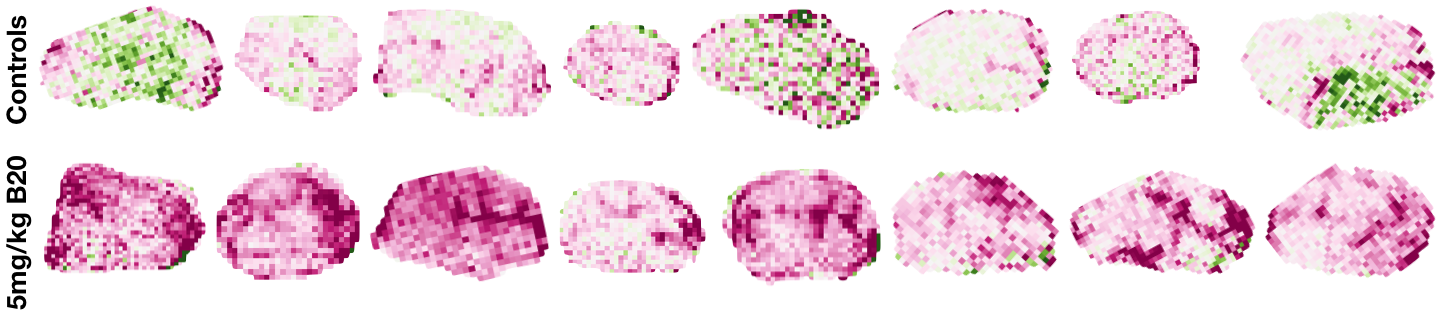
\includegraphics[width=\textwidth]{oemri_thesis3/oemri_thesis3-images/1_aarts3_b20_dOEMRI.png} % requires the graphicx package
   \caption{Normalized weighting factor maps obtained from ICA (dOE-MRI maps) are shown for control tumours as well as those treated with 5mg/kg B20 and imaged 48 hours later.
   Of the 10-16 slices for each animal, a representative slice was chosen.
   As indicated by the distribution of purple voxels, control tumours show considerably less response to oxygen than the treated tumours.
   Additionally, regions marked in green are considered to be hypoxic; these regions were not prevalent in the treated tumours.}
   \label{dOEMRImaps}
\end{figure}

\begin{figure}[htbp]
   \centering
   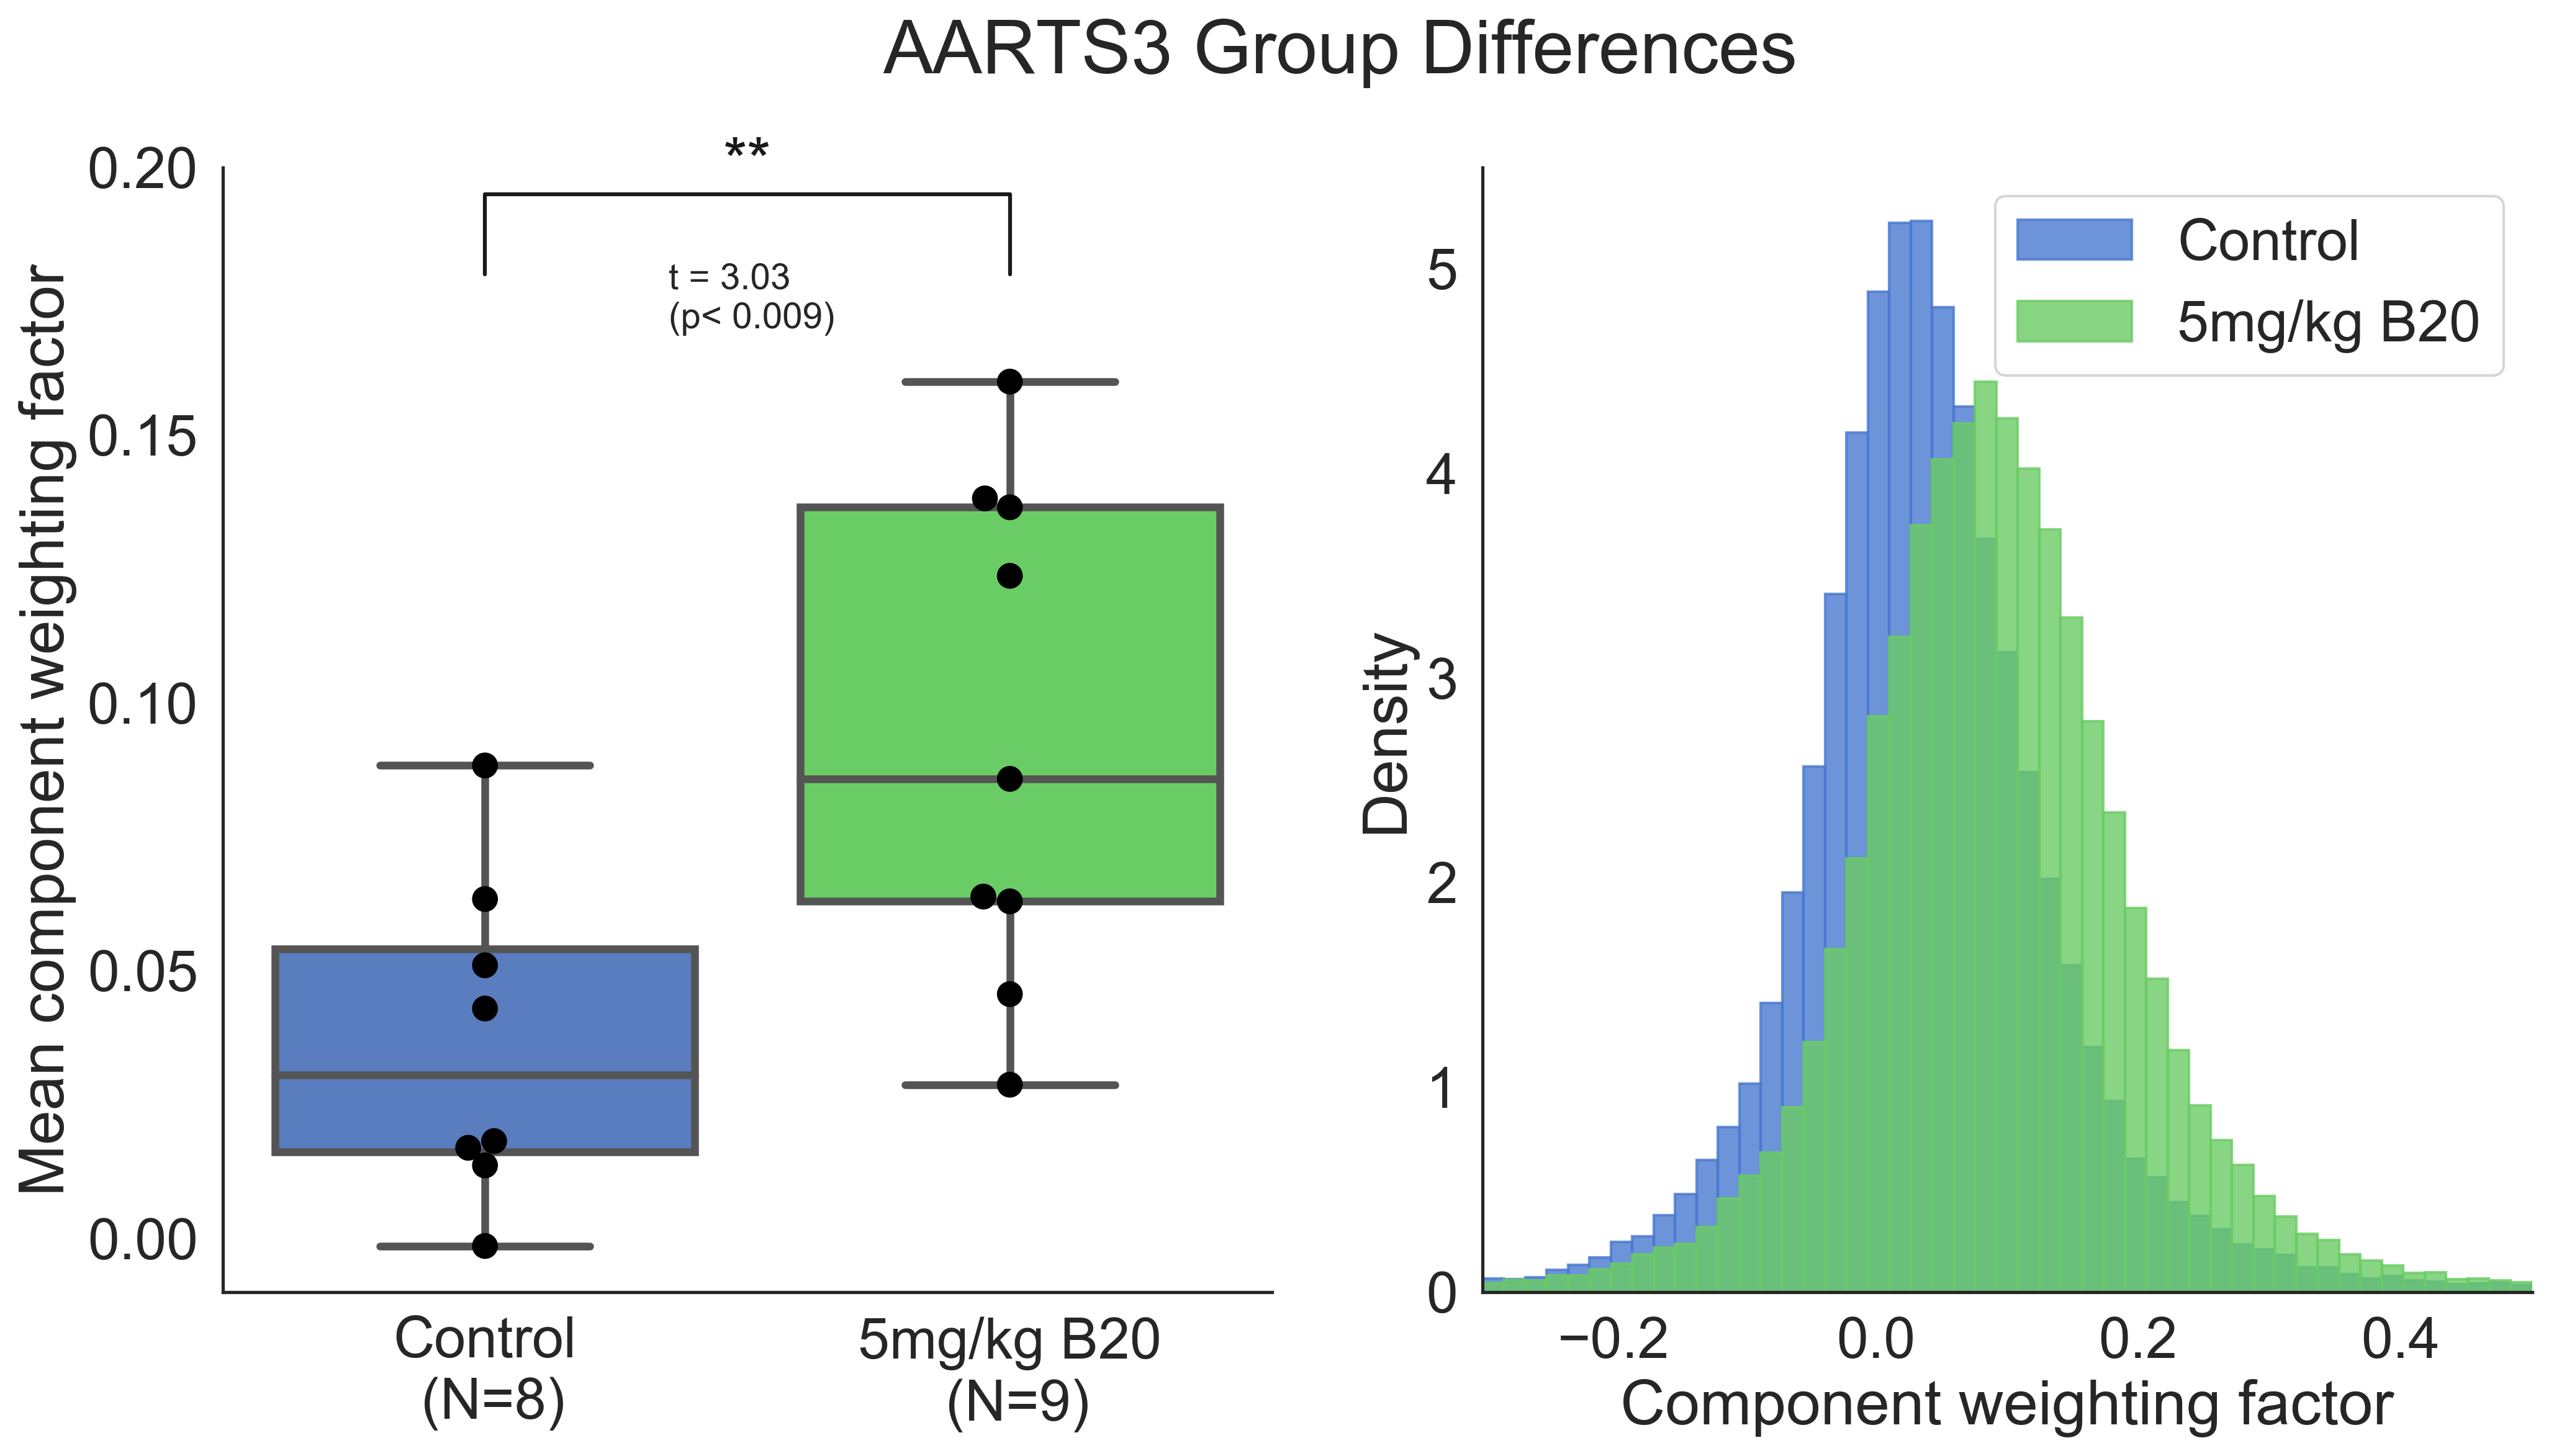
\includegraphics[width=0.7\textwidth]{oemri_thesis3/oemri_thesis3-images/2_aarts3_b20_boxplot_dOEMRI.png} % requires the graphicx package
   \caption{A) Group differences of the normalized mean component weighting factors from dOE-MRI are shown in a box plot.
   Each dot on the boxplot indicates the mean value of each mouse with the controls in blue and the treated in green.
   The differences are statistically significantly different (p=0.0092) with a large effect size (Hedge's g = 1.08).
   B) Density distributions of all voxels shows treated tumours shifting towards increased responsiveness to delivered oxygen (higher component weighting factor).}
   \label{aarts3boxplot}
\end{figure}

\subsection{SCCVII tumours implanted intramuscularly exhibit features different from those implanted subcutaneously}

\begin{figure}[htbp]
   \centering
   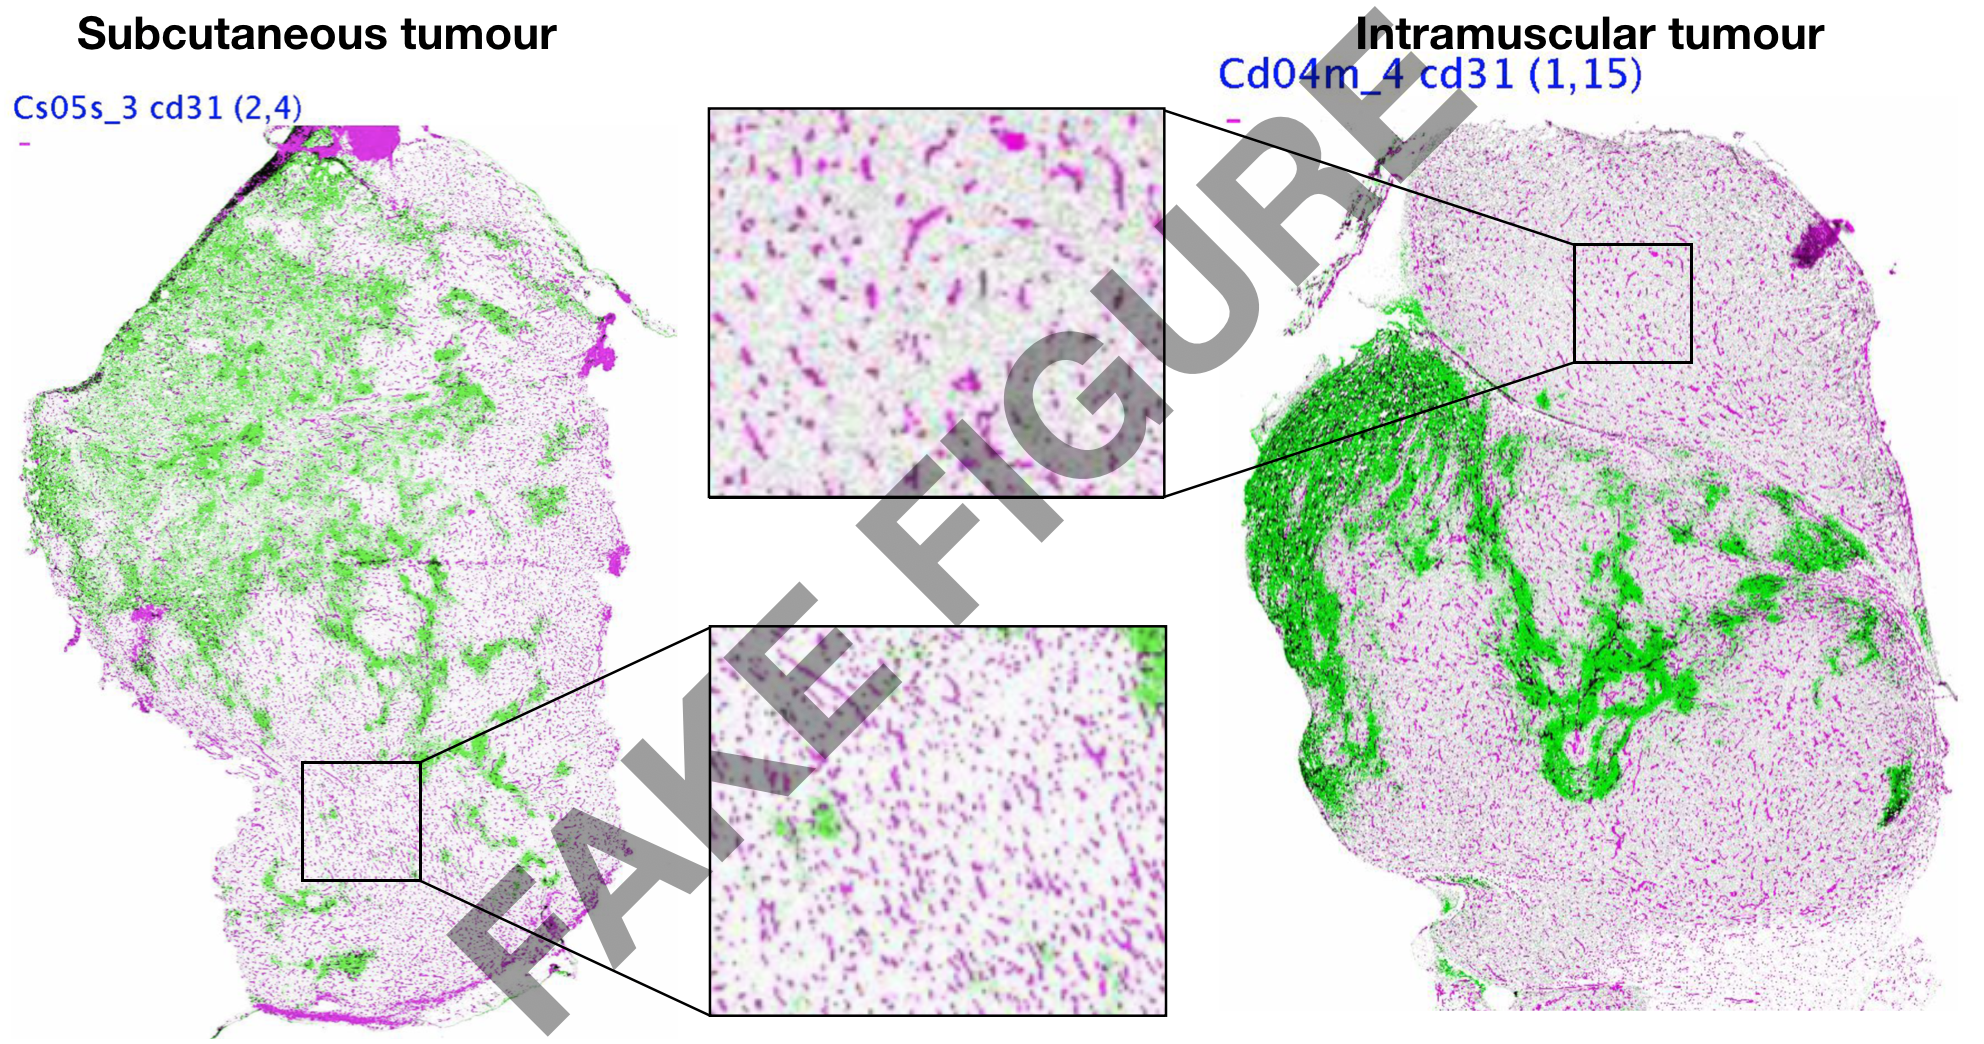
\includegraphics[width=\textwidth]{oemri_thesis3/oemri_thesis3-images/3_imsc_zoomed.png} % requires the graphicx package
   \caption{example caption}
   \label{imsc}
\end{figure}

The location of tumour cell implants in a mouse has a large bearing on the microenvironment of the resulting  xenograft, as access to surrounding normal tissue vasculature, and the overall growth environment plays a large role in tumour progression [refs]~\todo[backgroundcolor=green]{need refs here}. 
For the same concentration of cells implanted, IM tumours typically~\todo[backgroundcolor=green]{Question about this posed in Mattermost: http://bit.ly/2S79mKm} grow much faster,~\todo[backgroundcolor=green]{You'd expect there'd be larger too but the controls are actually smaller than SC controls according to number of MR voxels. Fewer cells were implanted in the IM location?} have a more stable vascular architecture, less hypoxia (pimo staining), and increased vessel density (CD31 \%).
Fig.~\ref{imsc} highlights some of these differences in representative SCCVII  tumours implanted SC and IM. 
To evaluate whether oxygen responsiveness is altered as a consequence of these features, dOE-MRI was employed in mice bearing both SC and IM tumours.
Untreated mice with IM tumours were statistically significantly (Mann-WhitneyU test, p = 0.003) more responsive to oxygen compared to the subcutaneous tumours in the same mice (Fig.~\ref{OEP8boxplot}) and the effect size was moderate with Hedge's \emph{g}= 0.44.

\subsection{IM tumours are not more responsiveness to oxygen after B20 treatment}

Mean normalized component weighting factors from B20-treated IM tumours was 0.137$\pm$0.018, and control IM tumours was 0.146$\pm$0.017 and the groups were not statistically significantly different (Mann-WhitneyU test, p=0.42). 
Thus, the B20 treatment did not have a measurable effect on improving responsiveness to oxygen in IM tumours with a higher baseline oxygen responsiveness compared to subcutaneous tumours.
Histological data (Fig.~\ref{allHisto}) also indicates that control IM tumours have significantly less pimonidazole staining compared to SC controls.
Furthermore, reduction in pimonidazole staining between control and treated IM tumours is much lower than in SC tumours~\todo[backgroundcolor=green]{I should probably do more than a cursory check to make sure single SC tumours were similar to double SC tumours}. 
This provides clear evidence that the effects of B20 are highly dependent on the tumour microenvironment, which can be appropriately assessed \emph{in vivo} using dOE-MRI.
To ensure the SC tumours from mice with a double implant were similar to mice with only a single implant, three mice were implanted with subcutaneous tumours.
No differences were found (data not shown), so the SC tumours from this experiment were pooled together.
There was a statistically significant difference in mean component weighting factors between control (0.073 $\pm$0.009) and B20-treated (0.119 $\pm$0.013) subcutaneous tumours with a moderate effect size: Hedge's \emph{g}=0.44 (Fig.~\ref{OEP8boxplot}).

\begin{figure}[htbp]
   \centering
   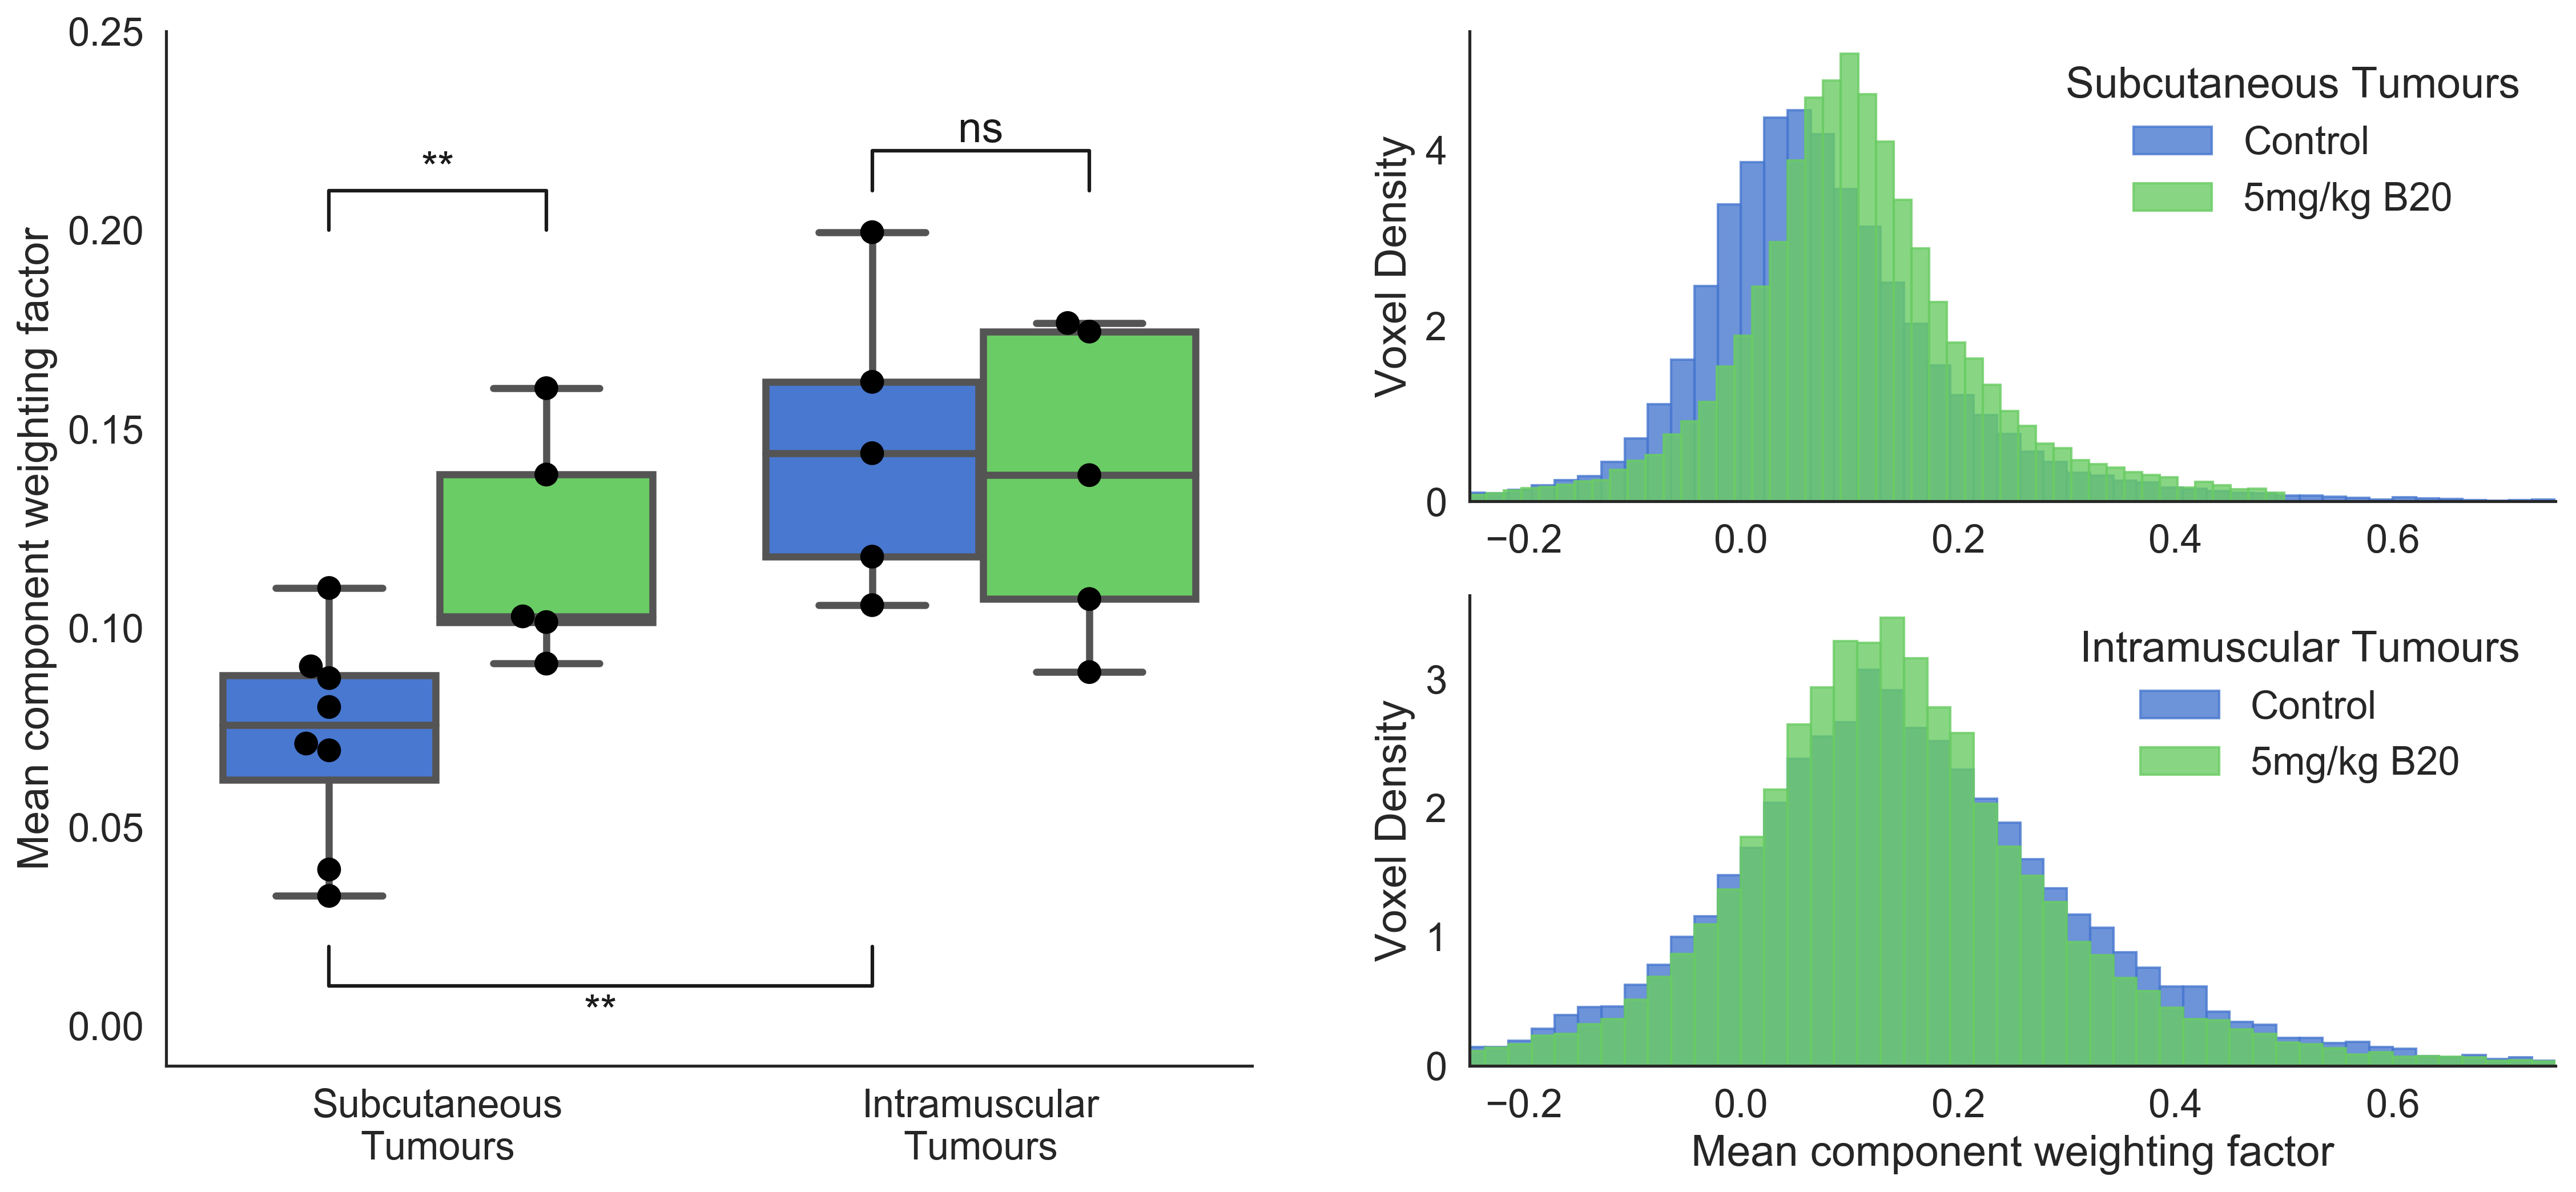
\includegraphics[width=\textwidth]{oemri_thesis3/oemri_thesis3-images/4_oep8_IMSC_b20_sanitized_dOEMRI.png} % requires the graphicx package
   \caption{\textbf{A)} Boxplot with four groups, 5mg/kg B20 treated and control mice with both SC and IM tumours.
   Differences between control SC and IM tumours, as well as control SC and treated SC tumours are statistically significant (Mann-WhitneyU test; p <0.005, marked as **).
   There was no significantly difference in treated and control IM tumours.
   \textbf{B)} Voxel density distributions of the normalized component weighting factors for SC (top) and IM (bottom) treated and control tumours.
   Note the shift of the IM control tumours towards a higher component weighting factor.}
   \label{OEP8boxplot}
\end{figure}

\begin{figure}[htbp]
   \centering
   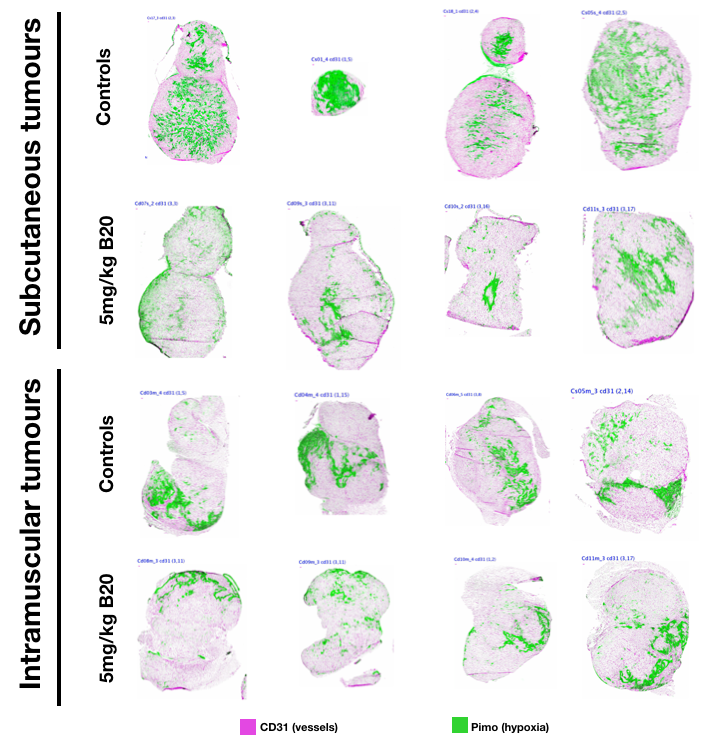
\includegraphics[width=\textwidth]{oemri_thesis3/oemri_thesis3-images/5_oep8_imsc_histo.png} % requires the graphicx package
   \caption{Representative histological sections from 16 total tumours of all four groups: 5mg/kg B20 treated and control mice with SC and IM tumours.
   Hypoxia marker pimonidazole staining is shown in green, and purple indicates the presence of blood vessels stained by CD31.}
   \label{allHisto}
\end{figure}

% \subsection{Comparing DCE-MRI perfusion patterns with dOE-MRI oxygenation patterns}

One SCCVII and one HCT-116 tumor-bearing mouse were catheterized and injected with 30mM solution of Gd-DTPA for DCE-MRI at a rate of 1mL/min using a power injector at a dose of 5$\mu$L/g.


\noindent\textbf{Perfusion maps:} Signal intensity timecourse from the DCE-MRI map was first normalized to the mean signal intensity pre-injection.
Area under the first 60 seconds of the normalized signal intensity enhancement curve after the injection was calculated (IAUC$_{60}$) using the composite Simpson's Rule (\texttt{scipy.integrate.simps}).
A binary ground-truth perfusion map was constructed by classifying all voxels with IAUC$_{60} > 0$ as perfused and everything else as unperfused.





% Where dOE-MRI and DCE-MRI scans were acquired in the same SCCVII and HCT-116 tumor-bearing mice,  maps of oxygenation status were compared to IAUC$_{60}$ perfusion maps, as shown in Figure~\ref{fig_perfusion}.
% Mean IAUC$_{60}$ for the well-perfused SCCVII tumor was 22 $\pm$ 16 \%$\cdot$s and for the comparatively poorly perfused HCT-116 tumor was 7$\pm$ 7 \%$\cdot$s.
% Well-oxygenated O$_2$-positive regions generally correspond to perfused, high IAUC$_{60}$ areas in both SCCVII and HCT-116 tumors.
% A large patch of necrosis, as identified in histological section, in the HCT-116 tumor was also extremely poorly perfused; such large patches of necrosis were not present in the SCCVII tumor.

% \begin{figure}[htbp]
%    \centering
%    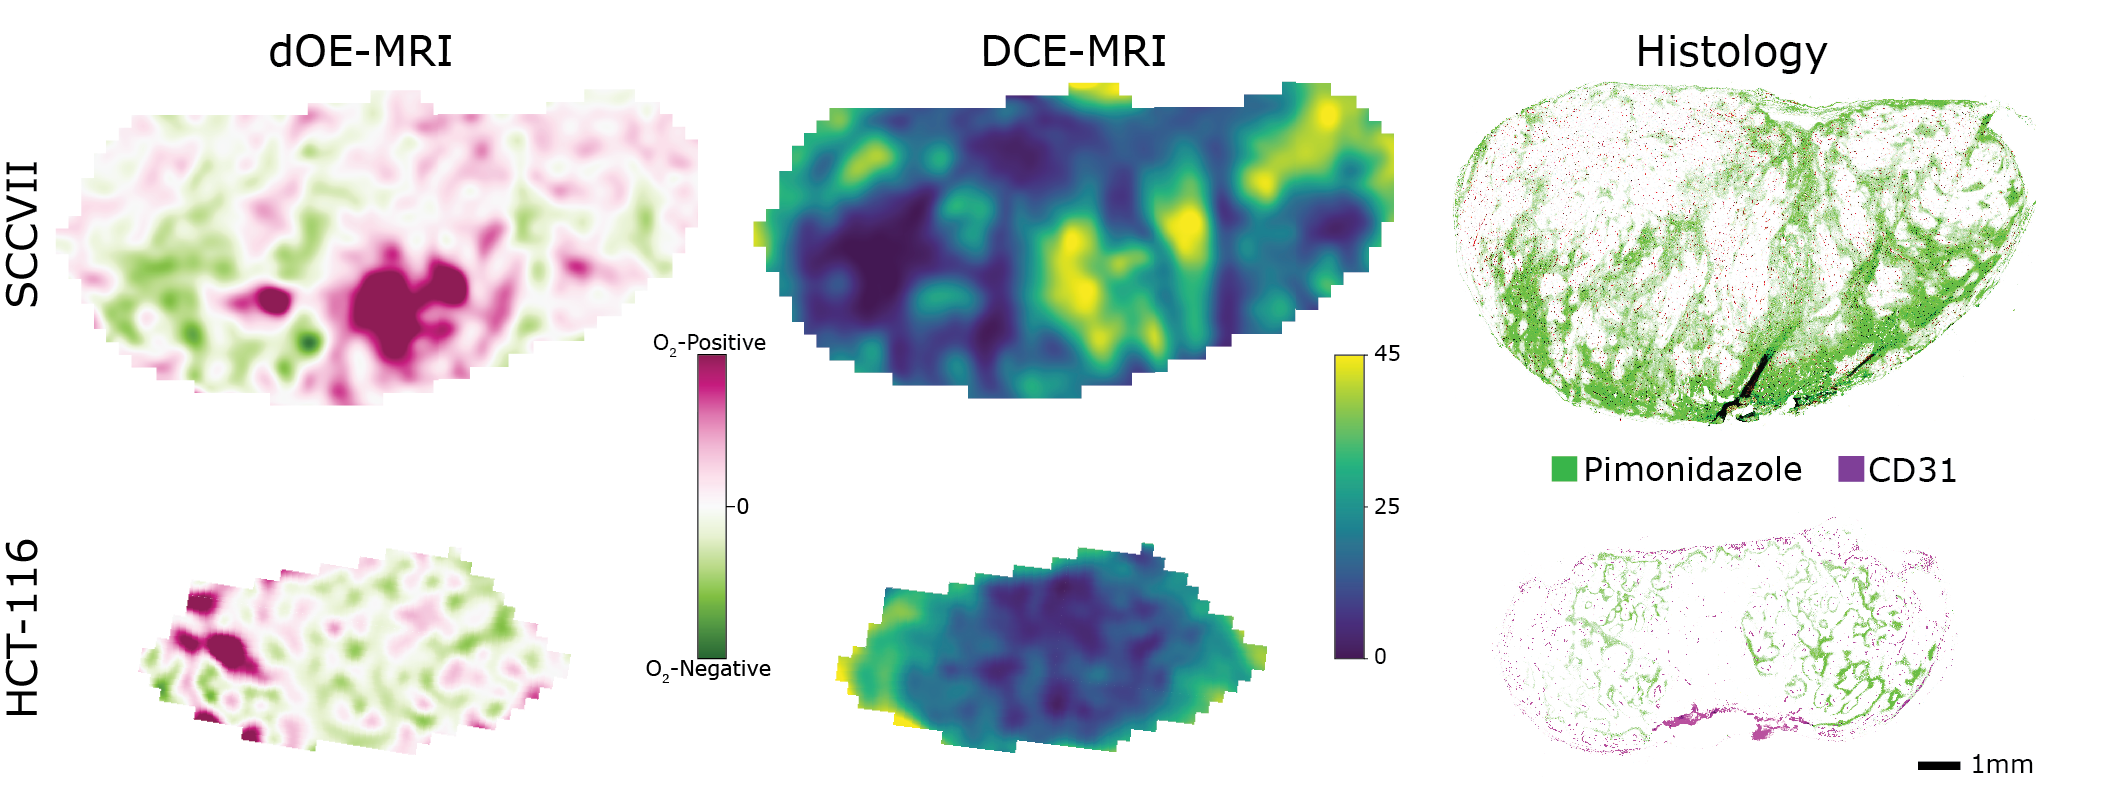
\includegraphics[width=\textwidth]{oemri_thesis3-images/fig_perfusion.eps} % requires the graphicx package
%    \caption{dOE-MRI maps and DCE-MRI IAUC$_{60}$maps and slice-matched histology sections of SCCVII and HCT-116 tumors. Large regions marked as purple in the dOE-MRI maps are O$_2$-positive and also correspond to regions that have high IAUC$_{60}$ values (yellow). Green or O$_2$-negative regions from the dOE-MRI map are often consistent with unperfused regions in the IAUC$_{60}$ (black), but there are regions of mismatch. Histology images stained with pimonidazole (green) and CD31 (purple) are shown for corresponding sections.
%    \label{fig_perfusion}}
% \end{figure}



\newpage

% ======================================================================
\section{Discussion}
% ======================================================================

Bevacizumab is a monocolonal antibody that targets the VEGF receptors on tumours and its effects have been widely reported~\cite{refs}.
Briefly, tumour xenografts receiving monocolonal antibodies to VEGF have consistently shown reductions in quantitative perfusion parameters from a variety of non-invasive imaging modalities including dynamic contrast enhanced (DCE) ultrasound (US)~\cite{Wang:2015bb}, DCE-MRI~\cite{OConnor:2009cg}, and micro PET~\cite{Nagengast:2007hx}.
For DCE-US, Wang et al. reported a significant reduction in peak enhancement, area under the curve, relative blood volume, and relative blood flow just 24 hours after a treatment of 10mg/kg of bevacizumab~\cite{Wang:2015bb} .  
With microPET, -----~\todo[backgroundcolor=green]{get details from nagegast reference}
Several DCE-MRI animal and human studies have shown reductions in Ktrans, vp, and ve after administration of antiangiogenic agents, including bevacizumab~\cite{mri}. \todo{cite also MR imaging biomarkers evaluating vascular normalization window after anti-vessel treatment}
Tumour growth delay data also clearly indicates that tumour growth is slowed after treatment with bevacizumab~\cite{growthdelay:junyang} and other similar VEGF inhibitors~\cite{sunitinib}.\todo{This does not sound right, is it really a vegf inhibitor?}

\textbf{discuss oxygenation effect of B20 on tumours}


\textbf{discuss IM vs. SC tumours}


\textbf{}





It has also been shown that tumour T1 is reduced following treatment with bevacizumab. 
However, to our knowledge, this is the first study showing oxygenation changes in tumours non-invasively using MRI. 


Sketch of Discussion:

\begin{itemize}
    \item Start with what's known about the effects of B20 on tumours
    \item Discuss existing human studies with DCE-MRI parameters talking Ktrans reduction after treatment
    \item Growth delays clearly show slowdown after B20 treatment, but it takes a few days
    \item Our data clearly shows an oxygenation improvement after administering B20; normalization hypothesis (cite Rakesh)
    \item Would be interesting to compare with DCE-MRI parameters and use multi-parametric MRI to try and understand what's going on 
    \item Interesting that tumour site has such a large bearing on oxygenation, worth considering for future experiments. 
    \item If the IM tumours were in patients and responded in such a way, one could conceivably not give them the drug which would have no effect and try a different one
    \item Briefly mention problems with T1weighting which could be a confounding factor
    \item Imperfect matches with pimonidazole
\end{itemize}

\subsection{random snippets}
O$_2$ positive or O$_2$-negative fractions are immune to this phenomenon, information about the level of response can be retained simply by applying the scaling factor when comparing scans at different temporal resolutions


% ======================================================================
\section{Conclusions}
% ======================================================================
Hello


